%! TeX program = lualatex
% \documentclass{beamer}
% \documentclass[handout]{beamer}
\documentclass[handout, notes]{beamer}
% \documentclass[handout, notes=only]{beamer}

\usetheme{metropolis}
\setbeamertemplate{section in toc}[sections numbered]

\usepackage{amsmath, amssymb, amsthm}
\usepackage{graphicx}
\usepackage{subfigure}
\usepackage{xcolor}
\usepackage[scr]{rsfso}
\usepackage{bm}

\graphicspath{{images/}}

\setlength{\parskip}{1.4em}
\setbeamertemplate{bibliography item}{\insertbiblabel}
\setbeamerfont{bibliography item}{size=\scriptsize}
\setbeamerfont{bibliography entry author}{size=\scriptsize}
\setbeamerfont{bibliography entry title}{size=\scriptsize}
\setbeamerfont{bibliography entry location}{size=\scriptsize}
\setbeamerfont{bibliography entry note}{size=\scriptsize}

% Sets

\newcommand{\C}{\mathbb{C}}
\newcommand{\R}{\mathbb{R}}
\newcommand{\Q}{\mathbb{Q}}
\newcommand{\Z}{\mathbb{Z}}
\newcommand{\N}{\mathbb{N}}


% Vectors and matrices

\newcommand{\vx}{\bm{x}}
\newcommand{\vy}{\bm{y}}
\newcommand{\vz}{\bm{z}}

\newcommand{\vX}{\bm{X}}
\newcommand{\vY}{\bm{Y}}
\newcommand{\vZ}{\bm{Z}}

\newcommand{\vO}{\bm{O}}

\newcommand{\vu}{\bm{u}}
\newcommand{\vv}{\bm{v}}
\newcommand{\vw}{\bm{w}}

\newcommand{\vmu}{\bm{\mu}}
\newcommand{\vth}{\bm{\theta}}

\newcommand{\I}{\mathbb{I}}


% Oversets

\newcommand{\tod}{\overset{d\,}{\longrightarrow}}
\newcommand{\topr}{\overset{p\,}{\longrightarrow}}
\newcommand{\toas}{\overset{a.s.\,}{\longrightarrow}}

\newcommand{\iid}{\overset{\text{iid}}{\sim}}

\newcommand{\eqd}{\overset{d}{=}}

% Distributions

\newcommand{\NN}{\mathcal{N}}
\newcommand{\UU}{\mathcal{U}}
\newcommand{\GG}{\mathcal{G}}

\newcommand{\Ell}{\operatorname{Ell}}


% Operators

\DeclareMathOperator{\tr}{trace}

\DeclareMathOperator{\E}{\mathbb{E}}

\DeclareMathOperator{\id}{id}

\DeclareMathOperator*{\argmax}{arg\,max}
\DeclareMathOperator*{\argmin}{arg\,min}

\DeclareMathOperator{\med}{med}
\DeclareMathOperator{\MAD}{MAD}

\DeclareMathOperator{\vol}{vol}
\DeclareMathOperator{\conv}{conv}

\DeclareMathOperator{\DD}{DD}
\DeclareMathOperator{\ReD}{ReD}
\DeclareMathOperator{\Sil}{Sil}

\DeclareMathOperator{\ET}{ET}
\DeclareMathOperator{\MHI}{MHI}
\DeclareMathOperator{\MEI}{MEI}

\DeclareMathOperator{\MBD}{MBD}
\DeclareMathOperator{\IQR}{IQR}

\DeclareMathOperator{\FO}{FO}
\DeclareMathOperator{\MO}{\textbf{MO}}
\DeclareMathOperator{\VO}{VO}
\DeclareMathOperator{\FOM}{FOM}
\DeclareMathOperator{\VOM}{VOM}

\DeclareMathOperator{\MOt}{MO}


% Brackets

\newcommand{\norm}[1]{\Vert #1 \Vert}
\newcommand{\ip}[2]{\langle #1, #2 \rangle}



\newcommand\blfootnote[1]{%
  \begingroup
  \renewcommand\thefootnote{}\footnote{#1}%
  \addtocounter{footnote}{-1}%
  \endgroup
}

\newcommand\Wider[2][4em]{%
\makebox[\linewidth][c]{%
  \begin{minipage}{\dimexpr\textwidth+#1\relax}
  \raggedright#2
  \end{minipage}%
  }%
}

\makeatletter
\patchcmd{\beamer@sectionintoc}
  {\vfill}
  {\vspace{0.1em}}
  {}
  {}
\makeatother


\title{
    Statistical Depth Functions
}
\author{
    Satvik Saha\\
    Supervised by Dr. Anirvan Chakraborty
}
\institute{
    Department of Mathematics and Statistics, \\
    Indian Institute of Science Education and Research, Kolkata
}
\date{17 May, 2024}

\begin{document}
    \maketitle


    \begin{frame}{Outline}
        \vspace{2em}
        \tableofcontents
    \end{frame}


    \begin{frame}{Depth Functions}
        A \emph{depth function} quantifies how \emph{central} a point $\bm{x}
        \in \mathscr{X}$ is with respect to a distribution $F$.

        This induces a \emph{center-outwards} ordering on the space
        $\mathscr{X}$.
    \end{frame}

    \begin{frame}{Depth Functions in $\R^d$}
        We want $D\colon \R^d \times \mathscr{F} \to \R$ to be bounded,
        non-negative, continuous, and satisfy the following properties.
        \begin{enumerate}
            \item[P1.] \textbf{Affine invariance:} $D(A\bm{x} + b, F_{A\bm{x} + b}) = D(\bm{x}, F_X)$.
            \item[P2.] \textbf{Maximality at centre:} $D(\theta, F_X) = \sup_{\bm{x} \in \R^d} D(\bm{x}, F)$.
            \item[P3.] \textbf{Monotonicity along rays:} $D(\bm{x}, F) \leq D(\theta + \alpha(\bm{x} - \theta), F)$.
            \item[P4.] \textbf{Vanish at infinity:} $D(\bm{x}, F) \to 0$ as $\Vert \bm{x} \Vert \to \infty$.
        \end{enumerate}
        \blfootnote{
            Zuo, Y., \& Serfling, R. (2000) General notions of statistical
            depth function
        }
    \end{frame}

    {
    \setbeamercolor{background canvas}{bg=white}
    \begin{frame}{The DD classifier}
        \Wider{
        \begin{figure}
        \begin{center}
            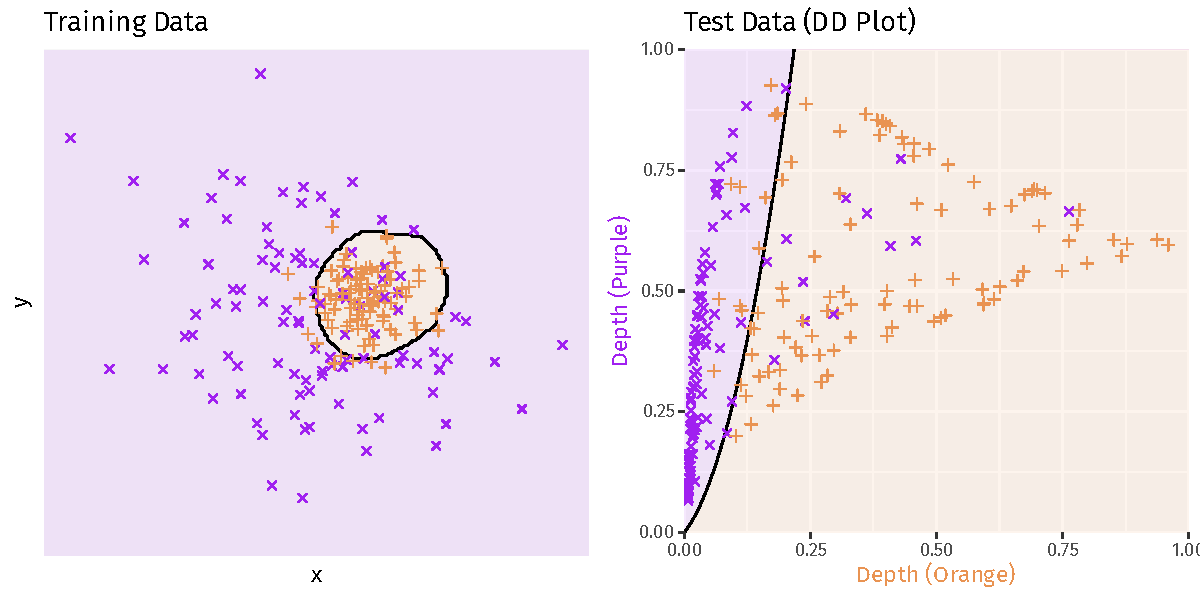
\includegraphics[width = \textwidth, page = 1]{classify}
        \end{center}
        \end{figure}
        }
    \end{frame}
    }


    \section{Depth Functions for Functional Data}

    {
    \setbeamercolor{background canvas}{bg=white}
    \begin{frame}{}
        \Wider{
        \begin{figure}
        \begin{center}
            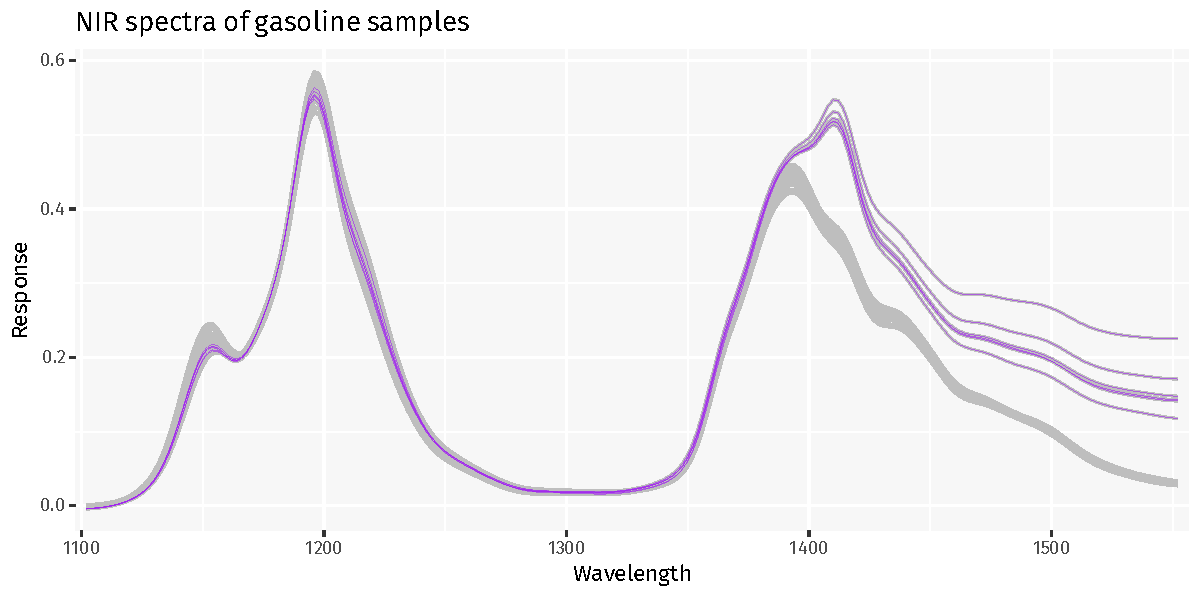
\includegraphics[width = \textwidth, page = 1]{octane}
        \end{center}
        \end{figure}
        }
    \end{frame}
    }


    \begin{frame}{Depth Functions in Banach spaces $\mathscr{X}$}
        Let $\mathscr{X}$ be a class of functions of the form $\vx\colon [0,
        1] \to \R^d$, equipped with a norm $\norm{\cdot}$.
        We typically choose $L^2[0, 1]$ or $\mathcal{C}[0, 1]$.

        We want to generalize the Zuo-Serfling properties (P1-4) in this
        setting, for depth functions $D\colon \mathscr{X} \times \mathscr{F}
        \to \R$.

        \blfootnote{
            Gijbels, I., \& Nagy, S. (2017) On a General Definition of Depth
            for Functional Data
        }
    \end{frame}

    \note{
        Properties $P3$ (Monotonicity along rays) and $P4$ (Vanish at
        infinity) carry over naturally.
    }

    \begin{frame}{Non-degeneracy}
        \begin{enumerate}
            \item[P0.] \textbf{Non-degeneracy:} $\inf_{\vx \in \mathscr{X}} D(\vx, F) < \sup_{\vx \in \mathscr{X}} D(\vx, F)$.
        \end{enumerate}

        The na\"ive generalization of the halfspace/Tukey depth \[
            D_H(\vx, F) = \inf_{\vv \in \mathscr{X}^*} P_{\vX \sim F}(\vv^*(\vX) \leq \vv^*(\vx)),
        \] is degenerate for a wide class of distributions $\mathscr{F}$.
        For instance, $\mathscr{X} = \mathcal{C}[0, 1]$, Gaussian processes with
        positive definite covariance kernels.

        \blfootnote{
            Chakraborty, A., \& and Chaudhuri, P. (2014) On data depth in
            infinite dimensional spaces
        }
    \end{frame}

    \note{
        This also applies to the functional analogue of the projection depth.
    }

    \begin{frame}{Non-degeneracy}

        The functional analogue of the spatial depth \[
            D_{Sp}(\vx, F) = 1 - \left\Vert\E_{\vX \sim F}\left[\frac{\vx - \vX}{\norm{\vx - \vX}_2}\right]\right\Vert_2,
        \] does not suffer from degeneracy.


        \blfootnote{
            Chakraborty, A., \& and Chaudhuri, P. (2014) The spatial
            distribution in infinite dimensional spaces and related quantiles
            and depths
        }
    \end{frame}


    \begin{frame}{Affine invariance}
        \begin{enumerate}
            \item[P1S.] \textbf{Scalar-affine invariance:} For $a, b \in \R$
            with $a$ non-zero and $\vx \in \mathscr{X}$, \[
                D(a\vx + b, F_{a\vX + b}) = D(\vx, F_{\vX}).
            \]
            \item[P1F.] \textbf{Function-affine invariance:} For $a, b, x \in
            \mathscr{X}$, with $ax \in \mathscr{X}$, \[
                D(ax + b, F_{aX + b}) = D(x, F_{X}).
            \]
        \end{enumerate}
    \end{frame}

    \begin{frame}{Maximality at center}
        We say that $F_{\vX}$ is symmetric about $\vth \in \mathscr{X}$ if for
        all $\varphi \in \mathscr{X}^*$, we have $\varphi(\vX)$ symmetric
        about $\varphi(\vth)$.

        \begin{enumerate}
            \item[P2C.] \textbf{Maximality at center of central symmetry:} For
            $F \in \mathscr{X}$ centrally symmetric about $\vth \in
            \mathscr{X}$, $D(\vth, F) = \sup_{\vx \in \mathscr{X}} D(\vx, F)$.

            \item[P2H.] \textbf{Maximality at center of halfspace symmetry:} For
            $F \in \mathscr{X}$ halfspace symmetric about $\vth \in
            \mathscr{X}$, $D(\vth, F) = \sup_{\vx \in \mathscr{X}} D(\vx, F)$.
        \end{enumerate}
    \end{frame}

    \begin{frame}{The Integrated and Infimal Depths}
        \[
            D_{FM}(\vx, F_{\vX}) = \int_{[0, 1]} D(\vx(t), F_{\vX(t)})\:w(t)\:dt.
        \]

        \[
            D_{Inf}(\vx, F_{\vX}) = \inf_{t \in [0, 1]} D(\vx(t), F_{\vX(t)}).
        \]

        \blfootnote{
            Fraiman, R., \& and Muniz, G. (2001) Trimmed means for functional
            data
        }
        \blfootnote{
            Mosler, K. (2013) Depth Statistics
        }
    \end{frame}

    \begin{frame}{The $J$-th order Integrated and Infimal Depths}
        \[
            D_{FM}^J(\vx, F_{\vX}) = \int_{[0, 1]^J} D((\vx(t_1), \dots, \vx(t_J))^\top, F_{(\vX(t_1), \dots, \vX(t_J))^\top})\:w(\bm{t})\:d\bm{t}.
        \]

        \[
            D_{Inf}^J(\vx, F_{\vX}) = \inf_{\bm{t} \in [0, 1]^J} D((\vx(t_1), \dots, \vx(t_J))^\top, F_{(\vX(t_1), \dots, \vX(t_J))^\top}).
        \]

        \blfootnote{
            Nagy, S., Gijbels, I., \& and Hlubinka, D. (2017) Depth-Based
            Recognition of Shape Outlying Functions
        }
    \end{frame}

    \note{
        These $J$-th order depths carry information about the derivatives of
        the curves, of orders $0, \dots, J - 1$.
    }


    \begin{frame}{The Band Depth}
        \[
            D_B^J(\vx, F) = \sum_{j = 2}^J P_{\vX_i \iid F}(\vx \in \conv(\vX_1, \dots, \vX_j)).
        \]

        This is the proportion of $j$-tuples of curves, for $2 \leq j \leq J$,
        which \emph{completely} envelope $\vx$.

        The band depth becomes degenerate for $\mathscr{X} = \mathcal{C}[0,
        1]$, Feller processes $\vX$ (e.g. Brownian motion) with $P(\vX_0 = 0)
        = 1$ and each $\vX_t$ for $t > 1$ non-atomic and symmetric about $0$.

        \blfootnote{
            L\'opez Pintado, S., \& Romo, J. (2009) On the concept of depth
            for functional data
        }
    \end{frame}

    \begin{frame}{The Modified Band Depth}
        Define the \emph{enveloping time} \[
            \ET(\vx; \vx_1, \dots, \vx_j) = m_1(\{t \in [0, 1]\colon \vx(t) \in \conv(\vx_1(t), \dots, \vx_j(t))\})
        \]

        The modified band depth is defined as \[
            D_{\MBD}(\vx, F) = \sum_{j = 2}^J \E_{\vX_i \iid F}\left[\ET(\vx; \vX_1, \dots, \vX_j)\right].
        \]
    \end{frame}

    \begin{frame}{The Half-Region Depth}
        We say that $\vy$ is in the hypograph (resp. epigraph) of $\vx$,
        denoted $\vy \in H_{\vx}$ (resp. $E_{\vx}$), if $\vy(t) \leq \vx(t)$
        (resp. $\geq$) for all $t \in [0, 1]$.

        The half-region depth is defined as \[
            D_{HR}(\vx, F) = \min\left\{P_F(H_{\vx}),\, P_F(E_{\vx})\right\}.
        \]

        This suffers from the same degeneracy problems as the band depth.

        \blfootnote{
            L\'opez Pintado, S., \& Romo, J. (2011) A half-region depth for
            functional data
        }
    \end{frame}

    \begin{frame}{The Modified Half-Region Depth}
        Define the Modified Hypograph (MHI) and Epigraph (MEI) Indices as
        \begin{align*}
            \MHI_F(\vx) &= \E_{\vX \in F}[m_1\{t \in [0, 1]\colon \vx(t) \geq \vX(t)\}], \\
            \MEI_F(\vx) &= \E_{\vX \in F}[m_1\{t \in [0, 1]\colon \vx(t) \leq \vX(t)\}].
        \end{align*}

        The modified half-region depth is defined as \[
            D_{MHR}(\vx, F) = \min\left\{\MHI_F({\vx}),\, \MEI_F({\vx})\right\}.
        \]
    \end{frame}


    \begin{frame}{Partially Observed Functional Data}
        Suppose that $\vX \sim F_{\vX}$ is not observed on the entire interval
        $[0, 1]$, but rather on some random compact subinterval $O \sim Q$
        (independent of $\vX$).

        Given a dataset $\mathscr{D} = \{(\vX_i, O_i)\}_{i = 1}^n$ where
        $(\vX_i, O_i) \iid F_{\vX} \times Q$, we keep track of the indices
        observed at time $t \in [0, 1]$ as $\mathscr{J}(t) = \{j\colon t \in
        O_j\}$, as well as their number $q(t) = |\mathscr{J}(t)|$.
    \end{frame}

    \begin{frame}{The Partially Observed Integrated Functional Depth (POIFD)}
        We may define a depth function in this setting via \[
            D_{POIFD}((\vx, o), F_{\vX} \times Q) = \int_{o} D(\vx(t), F_{\vX(t)}) \:w_o(t)\:dt,
        \] where $w_o(t) = q(t) / \int_0 q(t)\:dt$.

        \blfootnote{
            El\'ias, A., Jim\'enez, R., \& Shang, H. L. (2023) Depth-based
            reconstruction method for incomplete functional data
        }
    \end{frame}


    \begin{frame}{The functional reconstruction problem}
        Given $(\vX, O)$, can we estimate $\vX$ on $M = [0, 1]\setminus O$?

        We may search for a reconstruction operator $\mathcal{R}\colon L^2(O)
        \to L^2(M)$ that minimizes the mean integrated prediction squared
        error loss $\E[\norm{\vX_M - \mathcal{R}(\vX_O)}^2]$.
        In this setup, the best predictor is the conditional expectation
        $\E[\vX_M \mid \vX_O]$.

        We may also search for a continuous linear reconstruction operator
        $\mathscr{A}$, by estimating terms of the Karhunen-Lo\'eve expansion
        of $\vX$.
    \end{frame}


    \begin{frame}{The functional reconstruction problem}
        Another approach is to take a convex linear combination of curves from
        a suitable curve envelope with indices $\mathscr{I}$.

        The enveloping curves $\mathscr{I}$ may be chosen so that $(\vX, O)$
        is as deep as possible inside the curve envelope.

        Additionally, we want $\mathscr{I}$ to envelope $(\vX, O)$ for as long
        as possible (in the sense of the enveloping time $\ET$), and contain
        as many near curves (in an appropriately modified norm
        $\norm{\cdot}'$) to $(\vX, O)$ as possible.
    \end{frame}




    \section{Outlier detection for Functional Data}

    \begin{frame}{A na\"ive outlier detection scheme}
        Given data $\mathscr{D} = \{\vx_i\}_{i = 1}^n$, we may extract ranks
        $r_i = R(\vx_i, \hat{F}_n)$.

        For instance, we may choose \[
            R(\vx, \hat{F}_n) \;=\; \frac{1}{n} \sum_{i = 1}^n \bm{1}(D(\vx_i, \hat{F}_n) \leq D(\vx, \hat{F}_n)).
        \]

        Declare those $\vx_i$ with unusually high ranks $r_i$ as outliers, say
        greater than a cutoff $Q_3 + 1.5 \IQR$.
    \end{frame}


    {
    \setbeamercolor{background canvas}{bg=white}
    \begin{frame}{}
        \Wider{
        \begin{figure}
        \begin{center}
            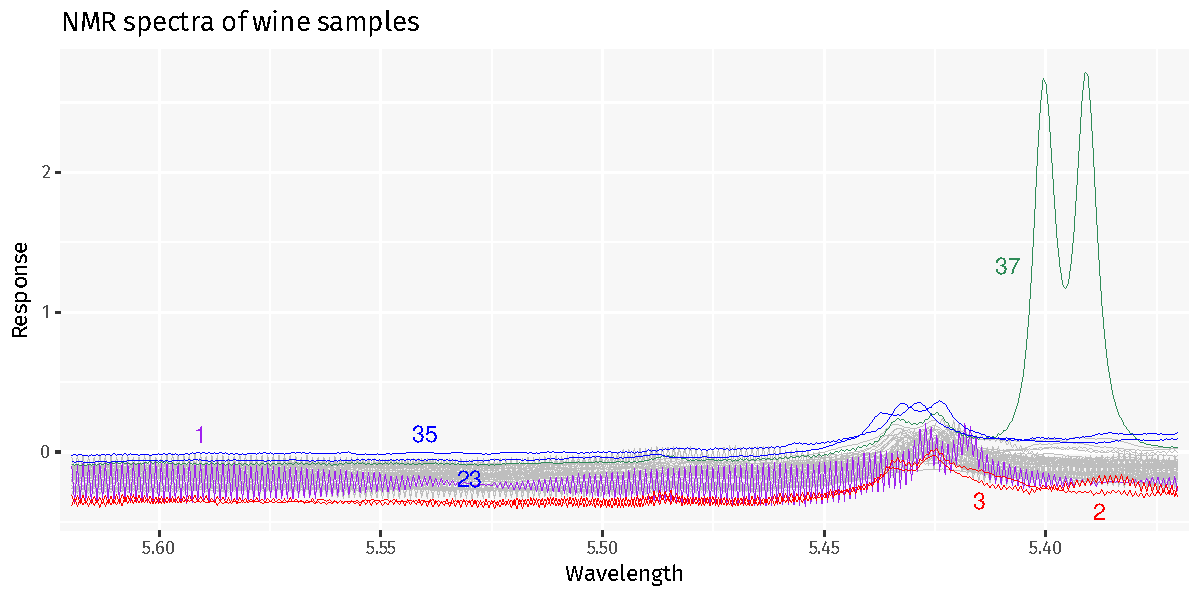
\includegraphics[width = \textwidth, page = 1]{wine}
        \end{center}
        \end{figure}
        }
    \end{frame}
    }

    \begin{frame}{Functional outliers}
        A curve $\vx\colon [0, 1] \to \R$ may exhibit outlying behaviour
        within a body of curves in many ways.

        \begin{itemize}
            \item \textbf{Isolated outlier:} Significant deviation over a
            short interval.
            \item \textbf{Persistent outlier:} Deviation over a large/entire
            interval.
            \begin{itemize}
                \item \textbf{Shape}
                \item \textbf{Shift}
                \item \textbf{Amplitude}
            \end{itemize}
        \end{itemize}

        \blfootnote{
            Hubert, M., Rousseeuw, P. J., \& Segaert, P. (2015) Multivariate
            functional outlier detection
        }
    \end{frame}

    \note{
        For a shape outlier, the slices $\vx(t)$ may all seem inconspicuous in
        the marginals $F_{\vX(t)}$.
    }

    \begin{frame}{Shape outliers and derivatives}
        One way of incorporating shape information of a curve $\vx$ is to
        bundle it with its derivatives $\vx^{(j)}$.

        \[
            \int_{[0, 1]} D((\vx^{(0)}(t), \dots, \vx^{(J)}(t))^\top, F_{(\vX^{(0)}(t), \dots, \vX^{(J)}(t))^\top})\:w(t)\:dt.
        \]
    \end{frame}

    \note{
        This suffers from errors in approximating derivatives, and the
        assumption of differentiability in the first place.
    }

    \begin{frame}{Shape outliers and the $J$-th order Integrated depth}
        We say that a curve $\vx$ is a $J$-th order outlier with respect to
        $F_{\vX}$ if there exists $\bm{t} \in [0, 1]^J$ such that the vector
        $(\vx(t_1), \dots, \vx(t_J))^\top$ is outlying with respect to
        $F_{(\vX(t_1), \dots, \vX(t_J))^\top}$.

        \[
            D_{FM}^J(\vx, F_{\vX}) = \int_{[0, 1]^J} D((\vx(t_1), \dots, \vx(t_J))^\top, F_{(\vX(t_1), \dots, \vX(t_J))^\top})\:w(\bm{t})\:d\bm{t}.
        \]

        \blfootnote{
            Nagy, S., Gijbels, I., \& and Hlubinka, D. (2017) Depth-Based
            Recognition of Shape Outlying Functions
        }
    \end{frame}

    \note[itemize]{
        \item This process looks at points of the form $(\vx(t), \vx(t + h),
        \dots)$, thus encoding information about the derivatives.

        \item One may choose the weight function $w(\cdot)$ to put emphasis on
        the diagonal.
    }


    \begin{frame}{The Centrality-Stability scheme}
        Consider an outlyingness function $O(\vx(t))$ which measures the
        outlyingness of $\vx(t)$ with respect to $F_{\vX(t)}$. For instance,
        we may choose \[
            O(\vx(t)) = \frac{\vx(t) - \med(\vX(t))}{\MAD(\vX(t))}.
        \]

        Then, we may define a depth function \[
            D(\vx, F_{\vX}) = \int_{[0, 1]} (1 + |O(\vx(t))|)^{-1} \:dt.
        \]

        \blfootnote{
            Hubert, M., Rousseeuw, P. J., \& Segaert, P. (2015) Multivariate
            functional outlier detection
        }
    \end{frame}

    {
    \setbeamercolor{background canvas}{bg=white}
    \begin{frame}{}
        \Wider{
        \begin{figure}
        \begin{center}
            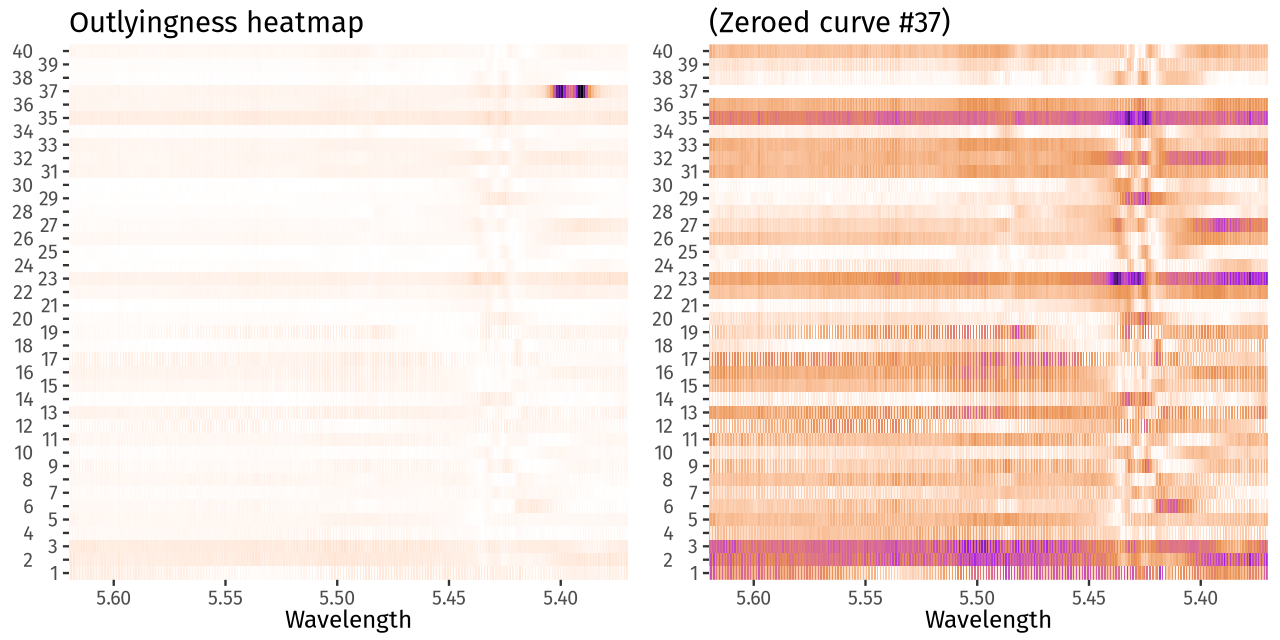
\includegraphics[width = \textwidth, page = 1]{outlyingness_heatmap_wine}
        \end{center}
        \end{figure}
        }
    \end{frame}
    }

    \begin{frame}{The Centrality-Stability scheme}
        Define \[
            \widetilde{MO}(\vx, F_{\vX}) = \int_{[0, 1]} |O(\vx(t))| \:dt
        \]

        Then, Cauchy-Schwarz gives \[
            D(\vx, F_{\vX}) \cdot (1 + \widetilde{MO}(\vx, F_{\vX})) \geq 1,
        \] with equality when $O(\vx(\cdot))$ remains constant over time.
    \end{frame}

    \begin{frame}{The Centrality-Stability scheme}
        Any sudden deviation in outlyingness will be detected by the
        \emph{stability deviation} \[
            \Delta S = (1 + \widetilde{MO}(\vx, F)) - \frac{1}{D(\vx, F)}.
        \]

        The \emph{centrality deviation} is measured as \[
            \Delta C = 1 - D(\vx, F).
        \]
    \end{frame}

    {
    \setbeamercolor{background canvas}{bg=white}
    \begin{frame}{}
        \Wider{
        \begin{figure}
        \begin{center}
            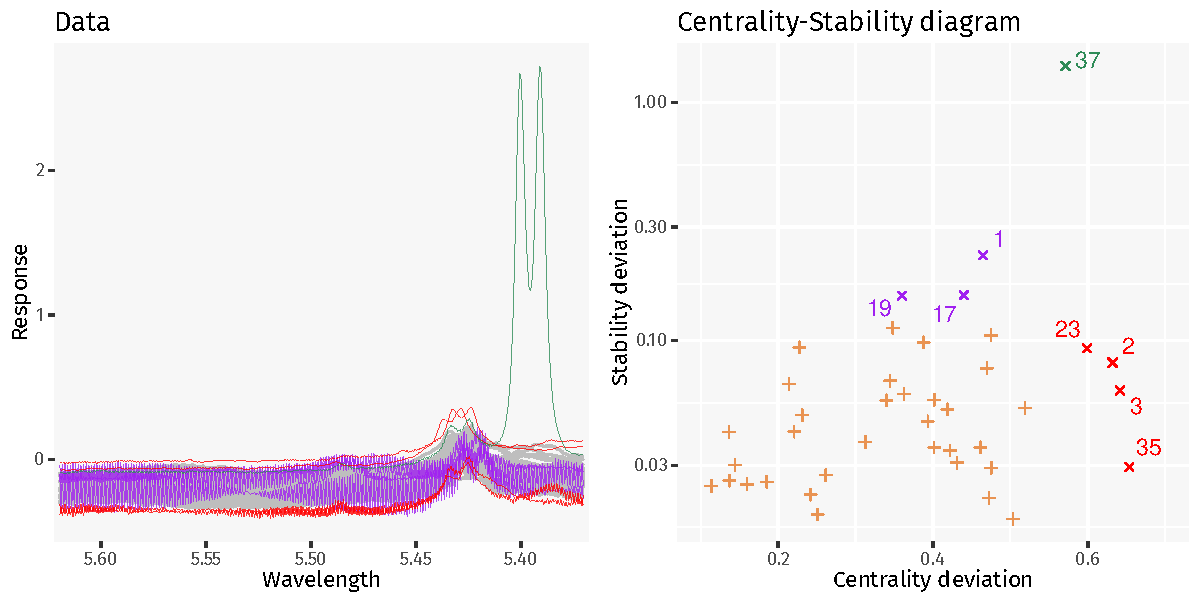
\includegraphics[width = \textwidth, page = 1]{centrality_stability_wine}
        \end{center}
        \end{figure}
        }
    \end{frame}
    }


    \begin{frame}{The MO-VO scheme}
        We may measure the variability in outlyingness over time more simply
        via
        \begin{align*}
            \MO(\vx, F) &= \int_{[0, 1]} O(\vx(t)) \:dt, \\
            \VO(\vx, F) &= \int_{[0, 1]} \norm{O(\vx(t)) - \MO(\vx, F)}^2 \:dt.
        \end{align*}

        \blfootnote{
            Dai, W., \& Genton, M. G. (2018) An outlyingness matrix for
            multivariate functional data classification
        }
    \end{frame}

    {
    \setbeamercolor{background canvas}{bg=white}
    \begin{frame}{}
        \Wider{
        \begin{figure}
        \begin{center}
            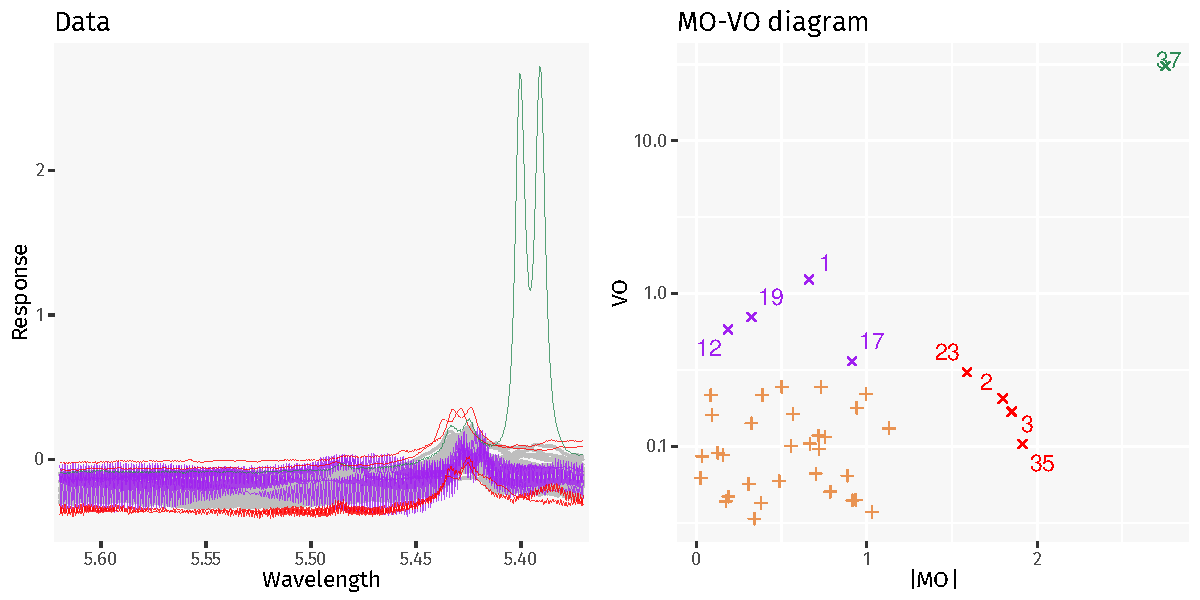
\includegraphics[width = \textwidth, page = 1]{MO_VO_wine}
        \end{center}
        \end{figure}
        }
    \end{frame}
    }

    \begin{frame}{The Outliergram}
        Given a dataset of curves $\mathscr{D} = \{\vx_i\}_{i = 1}^n$, the
        distances \[
            d_i = a_0 + a_1\MEI(\vx_i) + a_2 n^2 \MEI(\vx_i)^2 - \MBD(\vx_i),
        \] where $a_0 = a_2 = -2 / n (n + 1)$, $a_1 = 2(n + 1) / (n - 1)$, are
        indicative of shape outlyingness.

        Thus, one may declare $\vx_i$ as an outlier if $d_i$ exceeds a cutoff
        such as $Q_3 + 1.5\IQR$.

        \blfootnote{
            Arribas-Gil, A., \& Romo, J. (2014). Shape outlier detection and
            visualization for functional data: the outliergram
        }
    \end{frame}

    \note{
        The numbers $d_i$ are always positive!
    }

    {
    \setbeamercolor{background canvas}{bg=white}
    \begin{frame}{}
        \Wider{
        \begin{figure}
        \begin{center}
            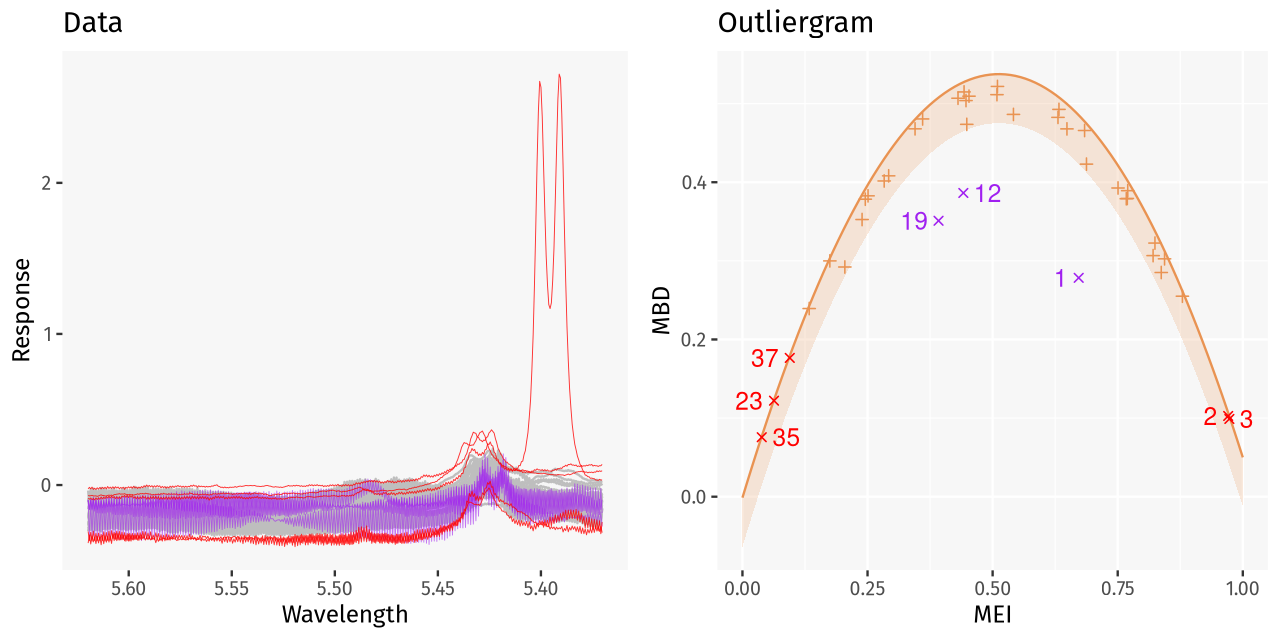
\includegraphics[width = \textwidth, page = 1]{outliergram_wine}
        \end{center}
        \end{figure}
        }
    \end{frame}
    }



    \section{Local Depth Functions}

    \begin{frame}{Elliptical distributions}
        We say that a distribution $F$ is elliptical if it admits a density of
        the form \[
            f_{\vX}(\vx) = c |\Sigma|^{-1/2} h\left((\vx - \vmu)^\top \Sigma^{-1} (\vx - \vmu)\right)
        \] for some strictly decreasing function $h$. Write $F \in \Ell(h;
        \vmu, \Sigma)$.

        An affine invariant depth function continuous in $\vx$ uniquely
        determines $F$ within $\Ell(h; \cdot, \cdot)$.
        The depth and density contours coincide.
    \end{frame}

    \note[itemize]{
        \item The whitened random variable $\vZ = \Sigma^{-1/2}(\vX - \vmu)$
        has density $f_Z(\vz) \propto h(\norm{\vz}^2)$.

        \item The halfspace, simplicial, projection depths satisfy this
        property.

        \item In general, depths such as the halfspace depth always produce
        convex central regions.
    }

    {
    \setbeamercolor{background canvas}{bg=white}
    \begin{frame}{}
        \Wider{
        \begin{figure}
        \begin{center}
            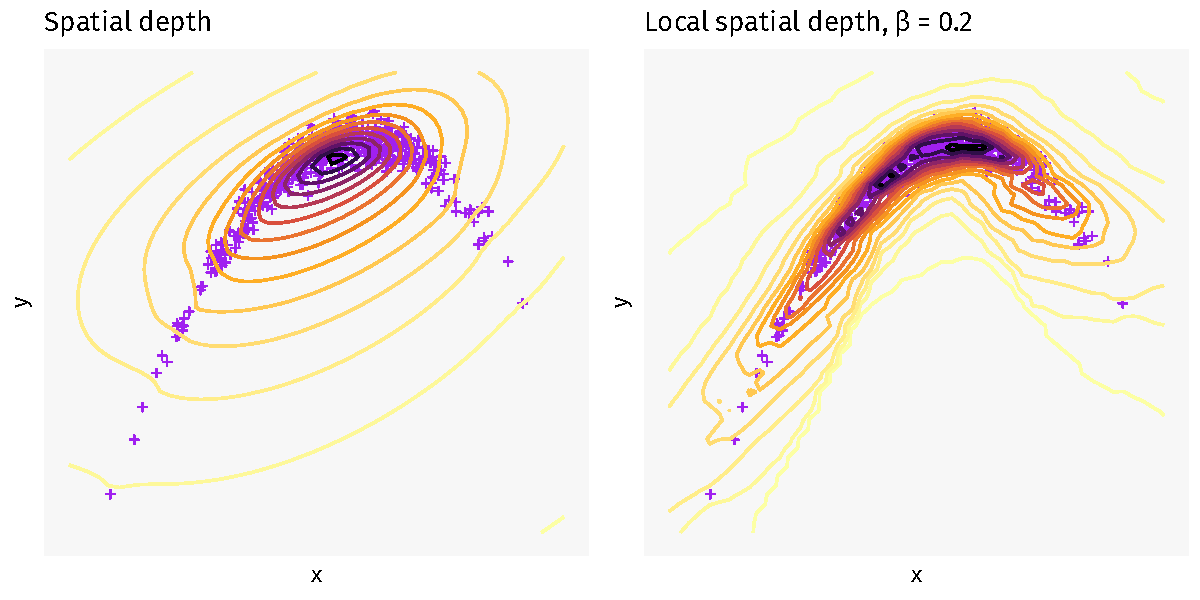
\includegraphics[width = \textwidth, page = 1]{localdepth_banana}
        \end{center}
        \end{figure}
        }
    \end{frame}
    }


    \begin{frame}{Local Depth neighbourhoods}
        Given $\vx \in \mathscr{X}$, we may symmetrize $F_{\vX}$ as \[
            F_{\vX}^{\vx} = \frac{1}{2} F_{\vX} + \frac{1}{2} F_{2\vx - \vX}.
        \]

        The probability-$\beta$ depth-based neighbourhood of $\vx$ in
        $F_{\vX}$ is simply the $\beta$-th central region of $F_{\vX}^{\vx}$.
        This is denoted by $N_{\beta}^{\vx}(F_{\vX})$.

        \blfootnote{
            Paindaveine, D., \& Van Bever, G. (2013) From depth to local
            depth: A focus on centrality
        }
    \end{frame}

    \begin{frame}{Local Depth}
        Let $F_\beta^{\vx}$ denote the distribution $F_{\vX}$ conditioned on
        $N_\beta^{\vx}(F_{\vX})$.

        The local depth function at locality level $\beta \in (0, 1]$ is
        defined as \[
            LD(\vx, F_{\vX}) = D(\vx, F_\beta^{\vx}).
        \]

        When $\beta = 1$, we have $LD_1 = D$.
    \end{frame}


    {
    \setbeamercolor{background canvas}{bg=white}
    \begin{frame}{}
        \Wider{
        \begin{figure}
        \begin{center}
            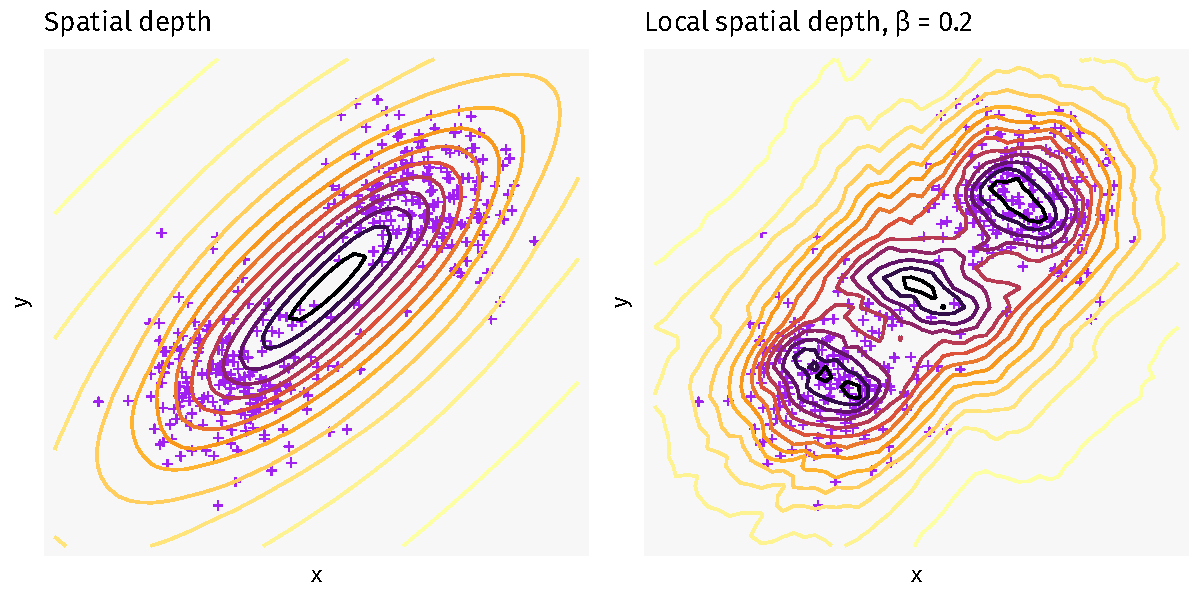
\includegraphics[width = \textwidth, page = 1]{localdepth_bimodal}
        \end{center}
        \end{figure}
        }
    \end{frame}
    }


    \begin{frame}{Local Depth based Regression}
        Let $\widetilde{F}_\beta^{\vx}$ denote the distribution
        $F_{\vX}^{\vx}$ conditioned on $N_\beta^{\vx}(F_{\vX})$.
        Note that this is angularly symmetric about $\vx$.

        Given $\vx \in \mathscr{X}$, we may define a local depth kernel,
        centered at $\vx$, via \[
            K_\beta^{\vx}\colon N_\beta^{\vx}(F_{\vX}) \to \R, \qquad
            \vz \mapsto D(\vz, \widetilde{F}_{\beta}^{\vx}).
        \] Extend this to $\mathscr{X}$ by setting $K_\beta^{\vx}(\cdot) = 0$
        outside $N_\beta^{\vx}(F_{\vX})$.
    \end{frame}

    \begin{frame}{Local Depth based Regression}
        We propose a linear estimator of the form \[
            \hat{\vy}_\beta(\vx) = \sum_i w_i(\vx) \vy_i, \qquad
            w_i(\vx) = \frac{K_\beta^{\vx}(\vx_i)}{\sum_j K_\beta^{\vx}(\vx_j)}.
        \]

        This may be interpreted as a weighted KNN estimator, or a variable
        bandwidth kernel estimator.

        We only have one tuning parameter $\beta \in (0, 1]$.
    \end{frame}

    {
    \setbeamercolor{background canvas}{bg=white}
    \begin{frame}{}
        \Wider{
        \begin{figure}
        \begin{center}
            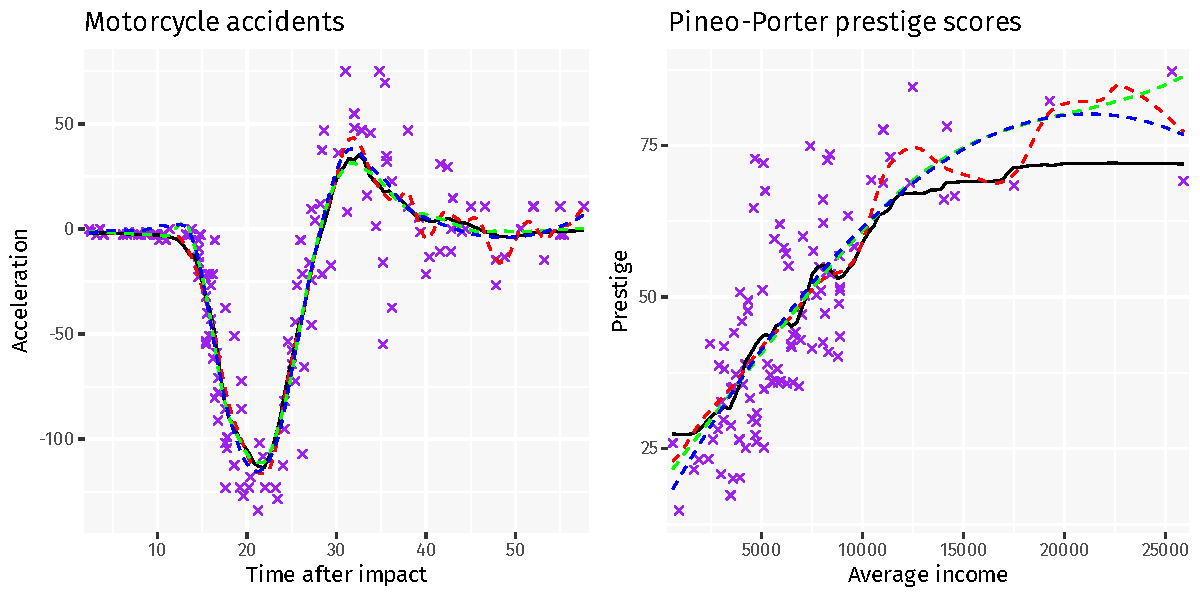
\includegraphics[width = \textwidth, page = 1]{localregression_univariate}
        \end{center}
        \end{figure}
        }
    \end{frame}
    }

    \note{
        The methods used are local depth based regression (black),
        Nadaraya-Watson kernel (red), local linear (green) and quadratic
        (blue).
    }


    {
    \setbeamercolor{background canvas}{bg=white}
    \begin{frame}{}
        \Wider{
        \begin{figure}
        \begin{center}
            \includegraphics[width = \textwidth, page = 5]{localregression_penntable_presentation}
        \end{center}
        \end{figure}
        }
    \end{frame}
    }

    {
    \setbeamercolor{background canvas}{bg=white}
    \begin{frame}{}
        \Wider{
        \begin{figure}
        \begin{center}
            \includegraphics[width = \textwidth, page = 2]{localregression_penntable_presentation}
        \end{center}
        \end{figure}
        }
    \end{frame}
    }

    {
    \setbeamercolor{background canvas}{bg=white}
    \begin{frame}{}
        \Wider{
        \begin{figure}
        \begin{center}
            \includegraphics[width = \textwidth, page = 3]{localregression_penntable_presentation}
        \end{center}
        \end{figure}
        }
    \end{frame}
    }

    {
    \setbeamercolor{background canvas}{bg=white}
    \begin{frame}{}
        \Wider{
        \begin{figure}
        \begin{center}
            \includegraphics[width = \textwidth, page = 4]{localregression_penntable_presentation}
        \end{center}
        \end{figure}
        }
    \end{frame}
    }



    \begin{frame}[allowframebreaks]{References}
        \nocite{*}
        \bibliographystyle{plain}
        \bibliography{references}
    \end{frame}

\end{document}
